\documentclass[draft]{agujournal2019}
\usepackage{url} %this package should fix any errors with URLs in refs.
\usepackage{lineno}
\usepackage{amsmath}
\usepackage{sidecap}
\usepackage[inline]{trackchanges} %for better track changes. finalnew option will compile document with changes incorporated.
\usepackage{soul}
\linenumbers

\draftfalse

\journalname{Tectonics}


\begin{document}

\title{Laurentia in the earliest Neoproterozoic: new paleomagnetic constraint from the Jacobsville Formation}

\authors{Yiming Zhang\textsuperscript{1}, Blake Hodgin\textsuperscript{1}, Nicholas Swanson-Hysell\textsuperscript{1}, James Pierce\textsuperscript{1,2}, Anthony Fuentes\textsuperscript{1}}

\affiliation{1}{Department of Earth and Planetary Science, University of California, Berkeley, CA, USA}
\affiliation{2}{Department of Earth and Planetary Sciences, Yale University, CT, USA}

\correspondingauthor{Yiming Zhang}{yimingzhang@berkeley.edu}

\begin{keypoints}
\item A new paleomagnetic pole from the ca. 990 Ma Jacobsville Formation \item Laurentia crossed the equator in the latest Mesoproterozoic to earliest Neoproterozoic
\item The new pole indicates the Grenville Loop could be much younger than thought
\end{keypoints}


\begin{abstract}
The paleogeography of Laurentia in the late Proterozoic is central to global paleogeography due to its central position in the supercontinent Rodinia. We develop a new paleomagnetic pole from red beds of the ca. 990 Ma Jacobsville Formation which serves as a crucial anchor point for Laurentia's position in the earliest Neoproterozoic. High-resolution thermal demagnetization experiments resolve detrital remanent magnetizations that pass a conglomerate test. An inclination corrected paleomagnetic mean pole position from the Jacobsville Formation confirm continued plate motion of Laurentia across the equator in the late Mesoproterozoic to early Neoproterozoic. The new pole from the interior of Laurentia indicates the plate slowed down significantly following the onset of the Grenvillian orogenesis on its eastern margin. This pole's position and age indicate the paleomagnetic poles developed from the Grenville Province most likely record coherent plate motion after major continental collision during the initial assembly of the supercontinent Rodinia.
\end{abstract}

% \section*{Plain Language Summary}
% [ enter your Plain Language Summary here or delete this section]


\section*{Keywords}
Rodinia\\
Laurentia  \\
Paleogeography\\
Neoproterozoic\\
\

apparent polar wander path\\
Inclination shallowing\\
Grenville\\
Keweenawan superchron\\
Red bed\\

\section*{Introduction}

The extensively studied paleomagnetic records of the ca. 1109 Ma to 1084 Ma North American Midcontinent Rift (i.e. the Keweenawan Track) provide crucial constraints on the paleogeography of Laurentia in the Mesoproterozoic \cite{Swanson-Hysell2019a}. As a result, the Keweenawan Track has become a central record for reconstructing the initial development of the ancient supercontinent Rodinia \cite{2021a}. As the rifting ceased and subsequently inverted following the onset of the Grenvillian Orogeny on Laurentia's eastern margin (Fig. \ref{fig:Geologic_map}), magmatism in the interior of Laurentia entered a period of quiescence that could have lasted for as long as $\sim$300 Myr until the emplacement of the ca. 780 Ma Gunbarrel large igneous province \cite{Harlan2003a, Mackinder2019a}. Due to this magmatic gap, Laurentia and its conjugate continents' paleogeographic configuration in the late Mesoproterozoic to mid-Neoproterozoic has remained largely uncertain \cite{Swanson-Hysell2021c}.

\begin{figure*}[h!]
\centering
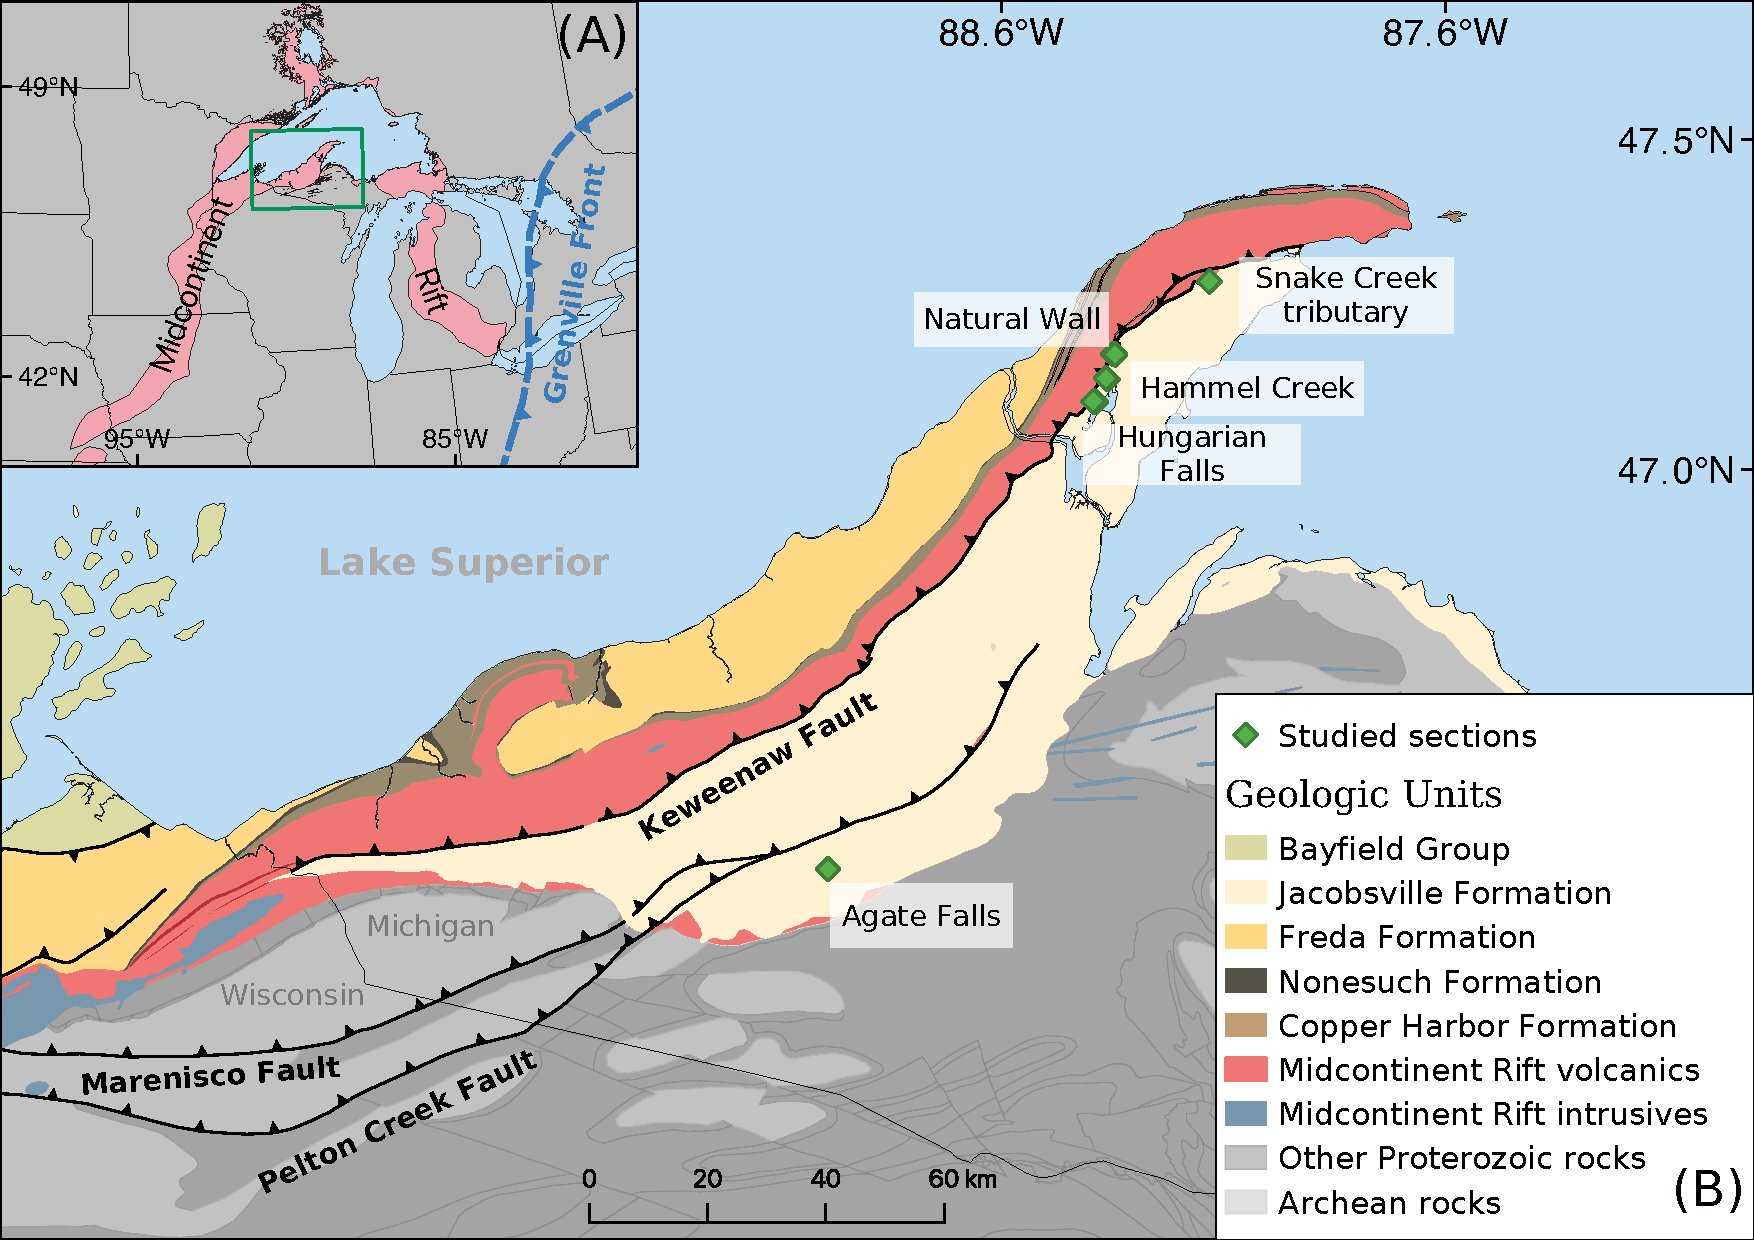
\includegraphics[width=\textwidth]{Geologic_map.pdf}
\caption{(A) Regional map showing location of the Grenville Front relative to the study area. The inset green box shows the extent of panel B. (B) Geologic map of northern Michigan and Wisconsin showing Midcontinent Rift igneous and sedimentary rocks, the Jacobsville Formation, other older Proterozoic rocks, and major post-rift thrust faults. Jacobsville stratigraphic sections along which paleomagnetic samples were collected in this study are shown as green diamond symbols.}
\label{fig:Geologic_map}
\end{figure*}

When igneous rock records are lacking, paleomagnetic data recorded by sedimentary rocks (e.g. red beds) can provide useful insights into the ancient geomagnetic field and record paleogeographic positions of sedimentary basins. In the Midcontinent Rift, the paleomagnetic poles developed from the ca. 1075 Ma Nonesuch Formation and the ca. 1070 Ma upper Freda Formation of the Oronto Group sediments that overlie the Midcontinent Rift volcanics in southern Lake Superior area (Fig. \ref{fig:Geologic_map}) provided crucial constraints for Laurentia's paleolatitude, orientation, and plate speed in the late Mesoproterozoic \cite{Henry1977a, Swanson-Hysell2019a, Rose2022a}. 

On top of the Oronto Group sediments overlies the post-rift Jacobsville Formation which was partly deformed during the inversion of the Midcontinent Rift (Fig. \ref{fig:Geologic_map}; \citeA{Hamblin1958a, Hodgin2022a, DeGraff2022a}). U-Pb detrital zircon ages and U-Pb calcite ages from the Keweenaw fault where the Jacobsville Formation is deformed against thrusted rift volcanics constrain the maximum depositional age of the Jacobsville Formation to be ca. 990 Ma \cite{Hodgin2022a}. The Jacobsville Formation contains abundant hematite-rich red beds which bear potential to further extend the apparent polar wander path (APWP) of Laurentia toward more recent times \cite{Hamblin1958a, Roy1978a}. Developing paleomagnetic data from the Jacobsville Formation will allow further development of Rodinia's paleogeographic evolution in the late Mesoproterozoic to early Neoproterozoic. 

Challenges exist in interpreting sedimentary paleomagnetic records. Primary detrital remanence acquired through settling and deposition of magnetic particles in the water column can be masked by secondary remanence acquired through precipitation and growth of new minerals within pore spaces of host sedimentary rocks syn- to post-deposition (e.g. pigmentary hematite). In red beds, it has been found that formation of the pigmentary hematite can significantly post-date the timing of sediment deposition, resulting in a chemical remanent magnetization (CRM) superimposed upon primary detrital remanent magnetization (DRM) carried by detrital grains \cite{Butler1992a}. To isolate the remanence components of the red beds of the Jacobsville Formation, \citeA{Roy1974a, Roy1978a} adopted a method first applied by \citeA{Collinson1965c} to preferentially remove fine-grained pigmentary hematite through prolonged immersion in concentrated HCl acid whereas leaving the coarser detrital grains that are more resistant to dissolution in place. Studies applying paired acid etching demagnetization and thermal demagnetization show that the pigmentary hematite grains tend to have lower unblocking temperatures than detrital ones \cite{Tauxe1980a, Bilardello2010c}. High-resolution thermal demagnetization experiments with temperature intervals as small as 1-2 \textdegree C have shown to be effective in isolating detrital remanence from chemical remanence as coarser hematite grains tend to have higher unblocking temperatures closer to the Ne\'el temperature of hematite \cite{Swanson-Hysell2019b}. In particular, a conglomerate test on a suite of fluvial intraclasts of the red beds in the Freda Formation shows that via thermal demagnetization one can isolate detrital magnetization vectors (which are reoriented in random directions in the clasts) from the secondary components carried by co-occurring authigenic hematite (which yield similar directions amongst clasts) \cite{Swanson-Hysell2019b}. 

Paleomagnetism of red beds has also been challenged by the controversial issue of correcting for inclination shallowing \cite{King1955a, Tauxe2004b, Bilardello2016b}. Due to rotation of detrital magnetic grains caused by authigenic processes such as compaction during lithification, inclinations recorded by sediments often have shallower angles than the local field in which they are deposited. To estimate the amount of inclination shallowing in a given package of sedimentary rocks, \citeA{Tauxe2004b} developed a statistical model (i.e. the elongation/inclination [E/I]method) that evaluates the deviation of the distribution of a large number ($>$100) of observed sedimentary paleomagnetic directional data with the predicted distribution given by a paleosecular variation model developed for the past 5 Myr (TK03) under the the geocentric axial dipole (GAD) hypothesis. Although the TK03 paleosecular variation model is based on data of relatively recent geomagnetic field variations, it has been shown to be compatible with data from the ca. 1.1 Ga lava flows of the Midcontinent Rift \cite{Tauxe2009a}. Further, \citeA{Pierce2022a} showed that the E/I method passes a field test for the 1.1 Ga Cut Face Creek Sandstone in the Midcontinent Rift as it successfully corrects the shallow paleomagnetic inclinations of the sediments to that of the North Shore Volcanic Group lava flows that bracket them. That study also further extended the method to better represent uncertainties associated with the amount of inclination shallowing when reporting sedimentary paleomagnetic pole positions by using the spherical elliptical Kent distribution \cite{Kent1982a} instead of the circular Fisher distribution \cite{Fisher1953a}. 

In this study, we investigate the hematite-bearing, fine-grained sandstone to siltstone lithofacies along five stratigraphic sections of the Jacobsville Formation on Keweenaw Peninsula, Michigan, USA. High-resolution thermal demagnetization isolate primary DRM from secondary CRM with the DRM passing a conglomerate test. We then use a paleomagnetic fold test to further constrain the timing of DRM acquisition in association with the structural inversion of the Midcontinent Rift. Finally, we develop a new inclination-corrected paleomagnetic pole for the Jacobsville Formation based on a large number of samples and investigate the paleo-continental configuration of Laurentia in the late Mesoproterozoic to early Neoproterozoic.


% The end of the ca. 1109 Ma to 1084 Ma intracontinental Midcontinent Rift magmatism and extension was marked by a transition to deposition of sedimentary rocks of the Oronto Group \cite{Ojakangas2001a} as the rift basin thermally subsided prior to the rift undergoing contractional deformation in the later stages of the Grenvillian orogeny \cite{Cannon1990b, Hodgin2022a}.

%  that has become central to the reconstruction of paleogeography of the assembly of supercontinent Rodinia. In addition to syn-rift rocks preservation, the cessation and later inversion of the rift allowed the development of syn-to post-rift basin development which accommodated the deposition of the ca. 1080 - 1050 Ma Oronto Group sedimentary rocks that are in total about 5 km thick. Overlying the Oronto Group is the Jacobsville formation which has been interpreted to be deposited in a back-bulge setting associated with the far-field propagation of the crustal-scale deformation caused by the Grenvillian Orogeny.

% A leading tectonic model for the cessation of the Midcontinent Rift and extension is that it occurred due to far-field compressional stress associated with the ca. 1090-980 Ma Grenvillian orogeny \cite{Cannon1990a}, when the collision of Laurentia with its conjugate margins led to the development of a back-bulge basin, accommodating the deposition of the Jacobsville Formation sediments as the inversion of the Midcontinent Rift progressed. Recent re-examination of the maximum deposition age of the Jacobsville Formation using zircon U-Pb whole grain chemical abrasion isotope dilution thermal ionization mass spectrometry has updated the maximum deposition age of the Jacobsville Formation to be ca. 990 Ma \cite{Hodgin2022a}. Such age constraint is consistent with backbulge subsidence model \cite{DeCelles, 2012}, indicating that the Jacobsville Formation may have been deposited in a Grenvillian foreland basin system that resulted from lithospheric flexure induced by orogenic loading \cite{Rivers2012a}. The relatively young age of the Jacobsville Formation compared to other Midcontinent Rift rocks makes the Jacobsville Formation an crucial target for further reconstructing the global paleogeography in the late Proterozoic. For further refining the paleogeographic connection between the poles of the Grenville Loop and those of the Keweenawan Track. 

% Paleomagnetic data for the Jacobsville Formation have led to a paleomagnetic pole position that appears to be a continuation of the Keweenawan Track from the Oronto Group poles (Roy and Robertson, 1978; Fig. 7; Table 4). As a result, its age has been interpolated to be latest Mesoproterozoic (e.g., 1020 Ma in Li et al., 2008) such that it was deposited prior to the ca. 1000 Ma Grenville loop poles. However, this age assignment has recently been questioned on the basis of laser-ablation–inductively cou- pled plasma–mass spectrometry (LA-ICP-MS) U-Pb detrital zircon dates from Jacobsville Sandstone samples. Malone et al. (2016) interpreted a maximum depositional age of 959 ± 19 Ma based on the weighted mean of the four youngest grains from 2050 LA-ICP-MS zircon dates. A similar age was proposed on the basis of the youngest LA-ICP-MS U-Pb dates in the study of Craddock et al. (2013). This young maximum interpreted age is intriguing because it suggests the unconformity above the Freda Sandstone spans at least 100 m.y. and was followed by continued sedimentation in the region long after rift activity. Nevertheless, the paleo- magnetic pole of the Jacobsville Sandstone (Roy and Robertson, 1978) appears to extend the Keweenawan Track from the Oronto Group poles in a manner that may be more consistent with deposition of the Jacobsville Formation in the late Mesoproterozoic. Given the conflict with this inferred age, the large uncertainty of individual LA-ICP-MS dates, and the possibility of outlier dates in such a large data set, it is beneficial to interpret the age of the youngest Jacobsville zircons dated CA-ID-TIMS to obtain more precise constraints. Using CA-ID-TIMS, a recent study by Hodgin et al (2022) redefines the maximum deposition age of the Jacobsville Formation as ca. 993 Ma.

% As the Midcontinent Rift magmatic activity wanes its strength and evolved into a failed intracontinental rift, Laurentia experienced a long period of magmatic quiescence in its interior, where basin subsidence dominated the rift basin. This was followed by the Grenville Orogeny, causing the the inversion of the rift along thrust belts such as the Keweenaw Fault (Fig. xxx). The lack of extensive magmatism from ca.1080 Ma to ca. 980 Ma in the Laurentia interior resulted in a significant gap (for at least 50 myr) of paleomagnetic poles between the Keweenawan Track (developed from interior Laurentia igneous and sedimentary rocks) and the Grenville Loop (poles developed from the Grenville Province rocks) (Fig. xxx; \cite{Swanson-Hysell2019a}).  

% Due to the lack of pmag records from the interior Laurentia, various hypotheses for the spatial relationship between the end of the Keweenawan Track and the Grenville Loop have been debated. One model argues for that the difference in pole locations indicates that the Grenville Province was once thousands of kilometers away from Interior Laurentia and was progressively approaching the southern margin of Laurentia in the late Mesoproterozoic \citep{Halls2015}. A corollary of this hypothesis is that there had to be a 4000 km shortening during the Grenville orogeny - colliding Amazonia-Laurentia. The other model favors that the Grenville Loop is a continuation of the Keweenawan Track - that the southerly continental drift of Laurentia continued across the equator onto the southern hemisphere from ca. 1070 Ma to ca.1000 Ma. and  approached this problem by developing data from metamorphosed dike and anorthosite and argued for Grenville  


\section*{Geologic settings}

\subsection*{Structure}
The ca. 1109 Ma to 1084 Ma North American Midcontinent Rift is a major intracontinental rift system that extends over 2000 km through the Laurentia craton (Fig. \ref{fig:Geologic_map}). However, the rifting failed to separate Laurentia into two continents. As its magmatism waned and thermal subsidence progressed in the rift basin, the $>$4 km of ca. 1085-1050 Ma Oronto Group sediments \cite{Fairchild2017a, Swanson-Hysell2019a} were deposited conformably on top of the rift volcanics (Fig. \ref{fig:Geologic_map}; \citeA{Cannon1989a}). Subsequently, the rift was inverted as the ca. 1090-980 Ma Grenvillian Orogeny commenced on the eastern margin of Laurentia (Fig. \ref{fig:Geologic_map}), eventually resulting in the propagation of far-field compressional stresses deep into the interior of Laurentia \cite{Cannon1993a, Cannon1994a}. 

During the rift inversion, Paleoproterozoic and Archean crust was uplifted via thrust faults such as the Marenisco fault and the Pelton Creek fault in the south, forming the crustal-scale Montreal River monocline (Fig. \ref{fig:Geologic_map}; \citeA{Cannon1993a}). The southern part of the post-rift Jacobsville Formation overlies an erosional angular unconformity that developed on lithologies that were exhumed through this earlier reverse motion (Fig. \ref{fig:Geologic_map}; \citeA{Hamblin1958a, Cannon1993a, Kalliokoski1982a}). North to these faults, Midcontinent Rift volcanic rocks were thrusted and folded along the Keweenaw fault which extends $\sim$250km from northern Wisconsin to northern Keweenaw Peninsula (Fig. \ref{fig:Geologic_map}; \citeA{DeGraff2022a}). Final inversion of the Keweenaw fault during the Rigolet phase of the Grenvillian Orogeny deformed part of the Jacobsville strata near the fault \cite{Hodgin2022a}. Recent mapping of the Jacobsville Formation also found that it can sometimes onlap the Midcontinent Rift volcanics within or adjacent to the Keweenaw Fault system near the northern end of the Keweenaw Peninsula (Fig. \ref{fig:Geologic_map}; \citeA{Tyrrell2019a, Mueller2021a}). 

Field observations find erosional contact and development of paleosol between the Jacobsville Formation and underlying volcanic rocks \cite{Hamblin1958a, Kalliokoski1975a}, and interpretations of seismic reflection data show that sedimentary rocks interpreted to be Jacobsville Formation lie unconformably on the Oronto Group \cite{Cannon1989a}. These data indicate that there was a prolonged period of sedimentation quiescence and net erosion between the end of Oronto Group deposition and onset of Jacobsville Formation deposition. Rb-Sr radiometric thermochronology data of \citeA{Cannon1993a} show the Montreal River monocline in which the Freda Formation and older basement rocks are deformed had been uplifted to mid to shallow crustal levels by ca. 1060 Ma. U-Pb dates of late kinematic calcite crystals that precipitated at ($\sim$50\textdegree C) in the hanging wall of the Keweenaw fault \cite{Hodgin2022a} indicate that by ca. 985 Ma the dominant inversion of Midcontinent Rift rocks along the Keweenaw fault has completed. Together, these data are consistent with the interpretation that the dominant inversion of the Midcontinent Rift basin happened during the ca. 1090-1020 Ma Ottawan phase of the Grenvillian Orogeny. They also indicate that the period of sedimentary quiescence in the rift basin may have lasted up to $\sim$70 Myrs from ca. 1060 to ca. 990 Ma. 

Syndepositional faulting that took place during Jacobsville deposition is inferred based on the observation of rift volcanic clasts within the Jacobsville basin. In the footwall of the Keweenaw fault near central Keweenaw Peninsula, strata of the Jacobsville Formation in contact with the Midcontinent volcanics are often steeply folded with the conglomeratic strata containing volcanic clasts \cite{Cannon1993a}. On the shore of Bete Grise Bay near the northeastern end of Keweenaw Peninsula, the Keweenaw fault is interpreted to have accommodated Grenville compressional stresses by forming a series of segmented en echelon thrusts \cite{Tyrrell2019a}. The timing of such faulting could be coeval with the deposition of the upper Jacobsville Formation, leading to the nonconformable onlapping of the Jacobsville sediments over the volcanics in addition to the thrust faulting relationship between the two units.

% at the same time when sediments from the older basement rocks along with distal input from the Grenville Province were deposited within the Jacobsville back-bulge basin system that in general wedges toward the northwest (Fig. \ref{fig:Geologic_map}; \cite{Hedgman2014a, Hodgin2022a}. 


\subsection{Sedimentary facies and general stratigraphy with interpretation}

% It has been interpreted that the Jacobsville Sandstone is equivalent to the Bayfield Group in northern Wisconsin, and the Fond Du Lac and Hinckley formations in Minnesota. Their shared lithofacies of basal conglomerate, cross-bedded fluvial fine to medium grained sandstone, and interbedded red micaceous siltstone could support the interpretation that these sedimentary rocks formed during a common period of post-rift basin formation following rift-related magmatism of the Midcontinent Rift. 
\begin{figure*}[h!]
\centering
\includegraphics[width=0.9\textwidth]{Field_photo.png}
\caption{\scriptsize Field photos of red beds of the Jacobsville Formation. At Baby Snake Creek and the Natural Wall ravine in northern Keweenaw Peninsula, intervals of red fine-grained sandstone to siltstone beds can be found through the steeply dipping to overturned basal strata near the Keweenaw fault (A,C) and also the nearly horizontal top strata (B,D). At Hungarian Falls, relatively thick intervals of red beds separated by hematite-depleted arenite to arkosic sandstones or conglomerates are found along a $>$100-meter-tall waterfall (E). Abundant reoriented siltstone rip-up clasts often exist within the conglomeratic layers above siltstone beds (F). Drill cores and block samples of these rip-up clasts were sampled for the paleomagnetic conglomerate test presented in Fig. \ref{fig:intraclast_pmag}. At Agate Falls, nearly flat-lying red fissile siltstone beds are exposed. (G). Subrounded detrital mica grains deposited parallel to the bedding plane are often associated with the siltstone facies. Another set of siltstone rip-up clasts were sampled from a conglomeratic layer near the basal exposure for the paleomagnetic conglomerate test. }
\label{fig:Field_photo}
\end{figure*}

The Jacobsville Formation is a fluvial sequence of feldspathic and quartzose conglomerates, sandstones, siltstones, and shales completely devoid of lava flows or cross-cutting igneous dikes although numerous  cross-cutting clastic dikes are present \cite{Hamblin1958a}. Sediments of the Jacobsville Formation is interpreted to be dominantly derived from the Oronto Group sediments and older basement rocks that were uplifted and deformed in the Montreal River monocline. The Jacobsville sediments are in general more quartz-rich than the Oronto Group sediments \cite{Hamblin1958a}. 

In the southern exposures of the Jacobsville Formation, abundant conglomerate facies typically have provenance sourced from Paleoproterozoic lithologies such as vein quartz and iron formation clasts \cite{Hamblin1958a, Kalliokoski1982a}. The occurrence of these conglomerates in proximity to the Marenisco fault and Pelton Creek faults is interpreted to represent syn-depositional development of local relief \cite{Kalliokoski1982a, Hedgman2014a}. Close to the Keweenaw Fault in central Keweenaw Peninsula (Fig. \ref{fig:Geologic_map}), the Jacobsville Formation consists dominantly of quartz-rich, cross-bedded, medium-grained sandstone, with locally abundant clast-supported pebble to cobble conglomerate, and interbeds of red, hematite-bearing, micaceous siltstone to fine-grained sandstone (Hungarian Falls, Hammell Creek, Natural Wall; Fig. \ref{fig:strat_column}). In this region, the conglomerate contains abundant volcanic clasts likely derived from uplifted Midcontinent Rift volcanics \cite{Irving1885a, Brojanigo1984a}. This clast-supported lithofacies can include siltstone rip-up clasts and sometimes channelized lenses of siltstones. More massive red beds also commonly interbed with hematite-depleted sandstone and conglomerate layers \cite<e.g.>{Hamblin1958a, Irving1885a}. The red beds typically appear brick-red to dark-red, consisting of fine-grained arenite to arkosic sandstone and siltstone sometimes with minor grey reduction spots (Fig. \ref{fig:Field_photo}). 

The occurrence of the rift volcanic-clast containing conglomeratic facies at Hungarian Falls, Hammell Creek, and Natural Wall indicates an interval of syn-depositional faulting in proximity to the Keweenaw fault in central part of the peninsula (Fig. \ref{fig:Geologic_map}, \ref{fig:strat_column}). Rapid weathering of the exhumed volcanics from the hanging wall also likely derived red clay and arkosic sandstone in the Jacobsville Formation which are most abundant near the fault but were also transported further away \cite{Hamblin1958a}. Rounded detrital mica grains commonly found within very fine, fissile siltstone strata are likely sourced from eroded Paleoproterozoic and Archean basement rocks in the Montreal River monocline highlands (Fig. \ref{fig:Geologic_map}). The mica grains can be up to $\sim$5mm in size (Fig. \ref{fig:Field_photo}). 

Thickness of the Jacobsville strata can vary significantly in northern Michigan \cite{Hamblin1958a, Kalliokoski1982a}, and complete stratigraphic sections are often not fully exposed at studied localities (Fig. \ref{fig:Geologic_map}). As a result, the exact stratigraphic association between sections of the Jacobsville Formation near central Keweenaw Peninsula and those exposed at Agate Falls and Baby Snake Creek is difficult to constrain. We propose one tentative stratigraphy model based on an interpreted Jacobsville sedimentary facies model. Given that deposition of conglomeratic facies was likely associated with syn-deposition faulting along the Keweenaw fault, this facies could have been deposited during the early stages of Jacobsville sedimentation, whereas siltstone and arkosic sandstone facies were probably deposited later with broader spatial distribution. Some early conglomeratic facies could have been reworked and contributed to the formation of Jacobsville red beds farther away from the fault. Based on this facies model, the relative lack of conglomerate facies at Agate Falls and at Baby Snake Creek, and field observations of onlapping Jacobsville Formation on top of previously deformed rift volcanics at Baby Snake Creek, could support an interpretation that Jacobsville sediments exposed at these two localities are slightly younger than the conglomerate-rich strata near central Keweenaw Peninsula (Fig. \ref{fig:Geologic_map}, \ref{fig:strat_column}). Further discussion regarding the stratigraphy in light of the paleomagnetic data is presented in section \ref{magstrat}. 

%At some point earlier on, we may need to articulate a facies model that can be used to justify the correlation scheme by 1) demonstrating that the conglomeratic facies at the grouped sites in the lower Keweenaw Peninsula, which are associated with siltstone deposition and arkosic sands, were likely deposited during an interval of syn-depositional faulting in proximity to the Keweenaw Fault; next 2) it can be suggested that rapid weathering of the exhumed basaltic rock from the hanging wall resulted in red clay most abundant to the fault but also deposited further away, and abundant partially weathering arkosic sands but which also occur farther away to some degree; 3) This interpretation is supported by the facies association being volcanic conglomerate, red siltstone, and arkosic sands (along with some other typical Jacobsville facies) and is the basis for suggesting that farther travelled silt and arkosic sands could be correlated with the conglomerates. Tentatively this stratigraphicaly significant and unique facies association may serve as a basis for correlation across the basin during a time of more significant syn-depositional fault uplift.


Overall, the extent of the Jacobsville Formation has been mapped along the lake shore of the Keweenaw Peninsula from northern Michigan, USA, to the north side of Michipicoten Island and perhaps to northern Sault Ste Marie, Canada (Fig. \ref{fig:Geologic_map}; \citeA{Hamblin1958a}). It has also been interpreted that the Jacobsville Formation could be temporally and lithologically correlated with the Bayfield Group sediments in northern Wisconsin and the Fond du Lac and Hinckley Formation in Minnesota \cite{Hamblin1958a, Kalliokoski1982a, Malone2016a}.


\begin{figure*}[h!]
\centering
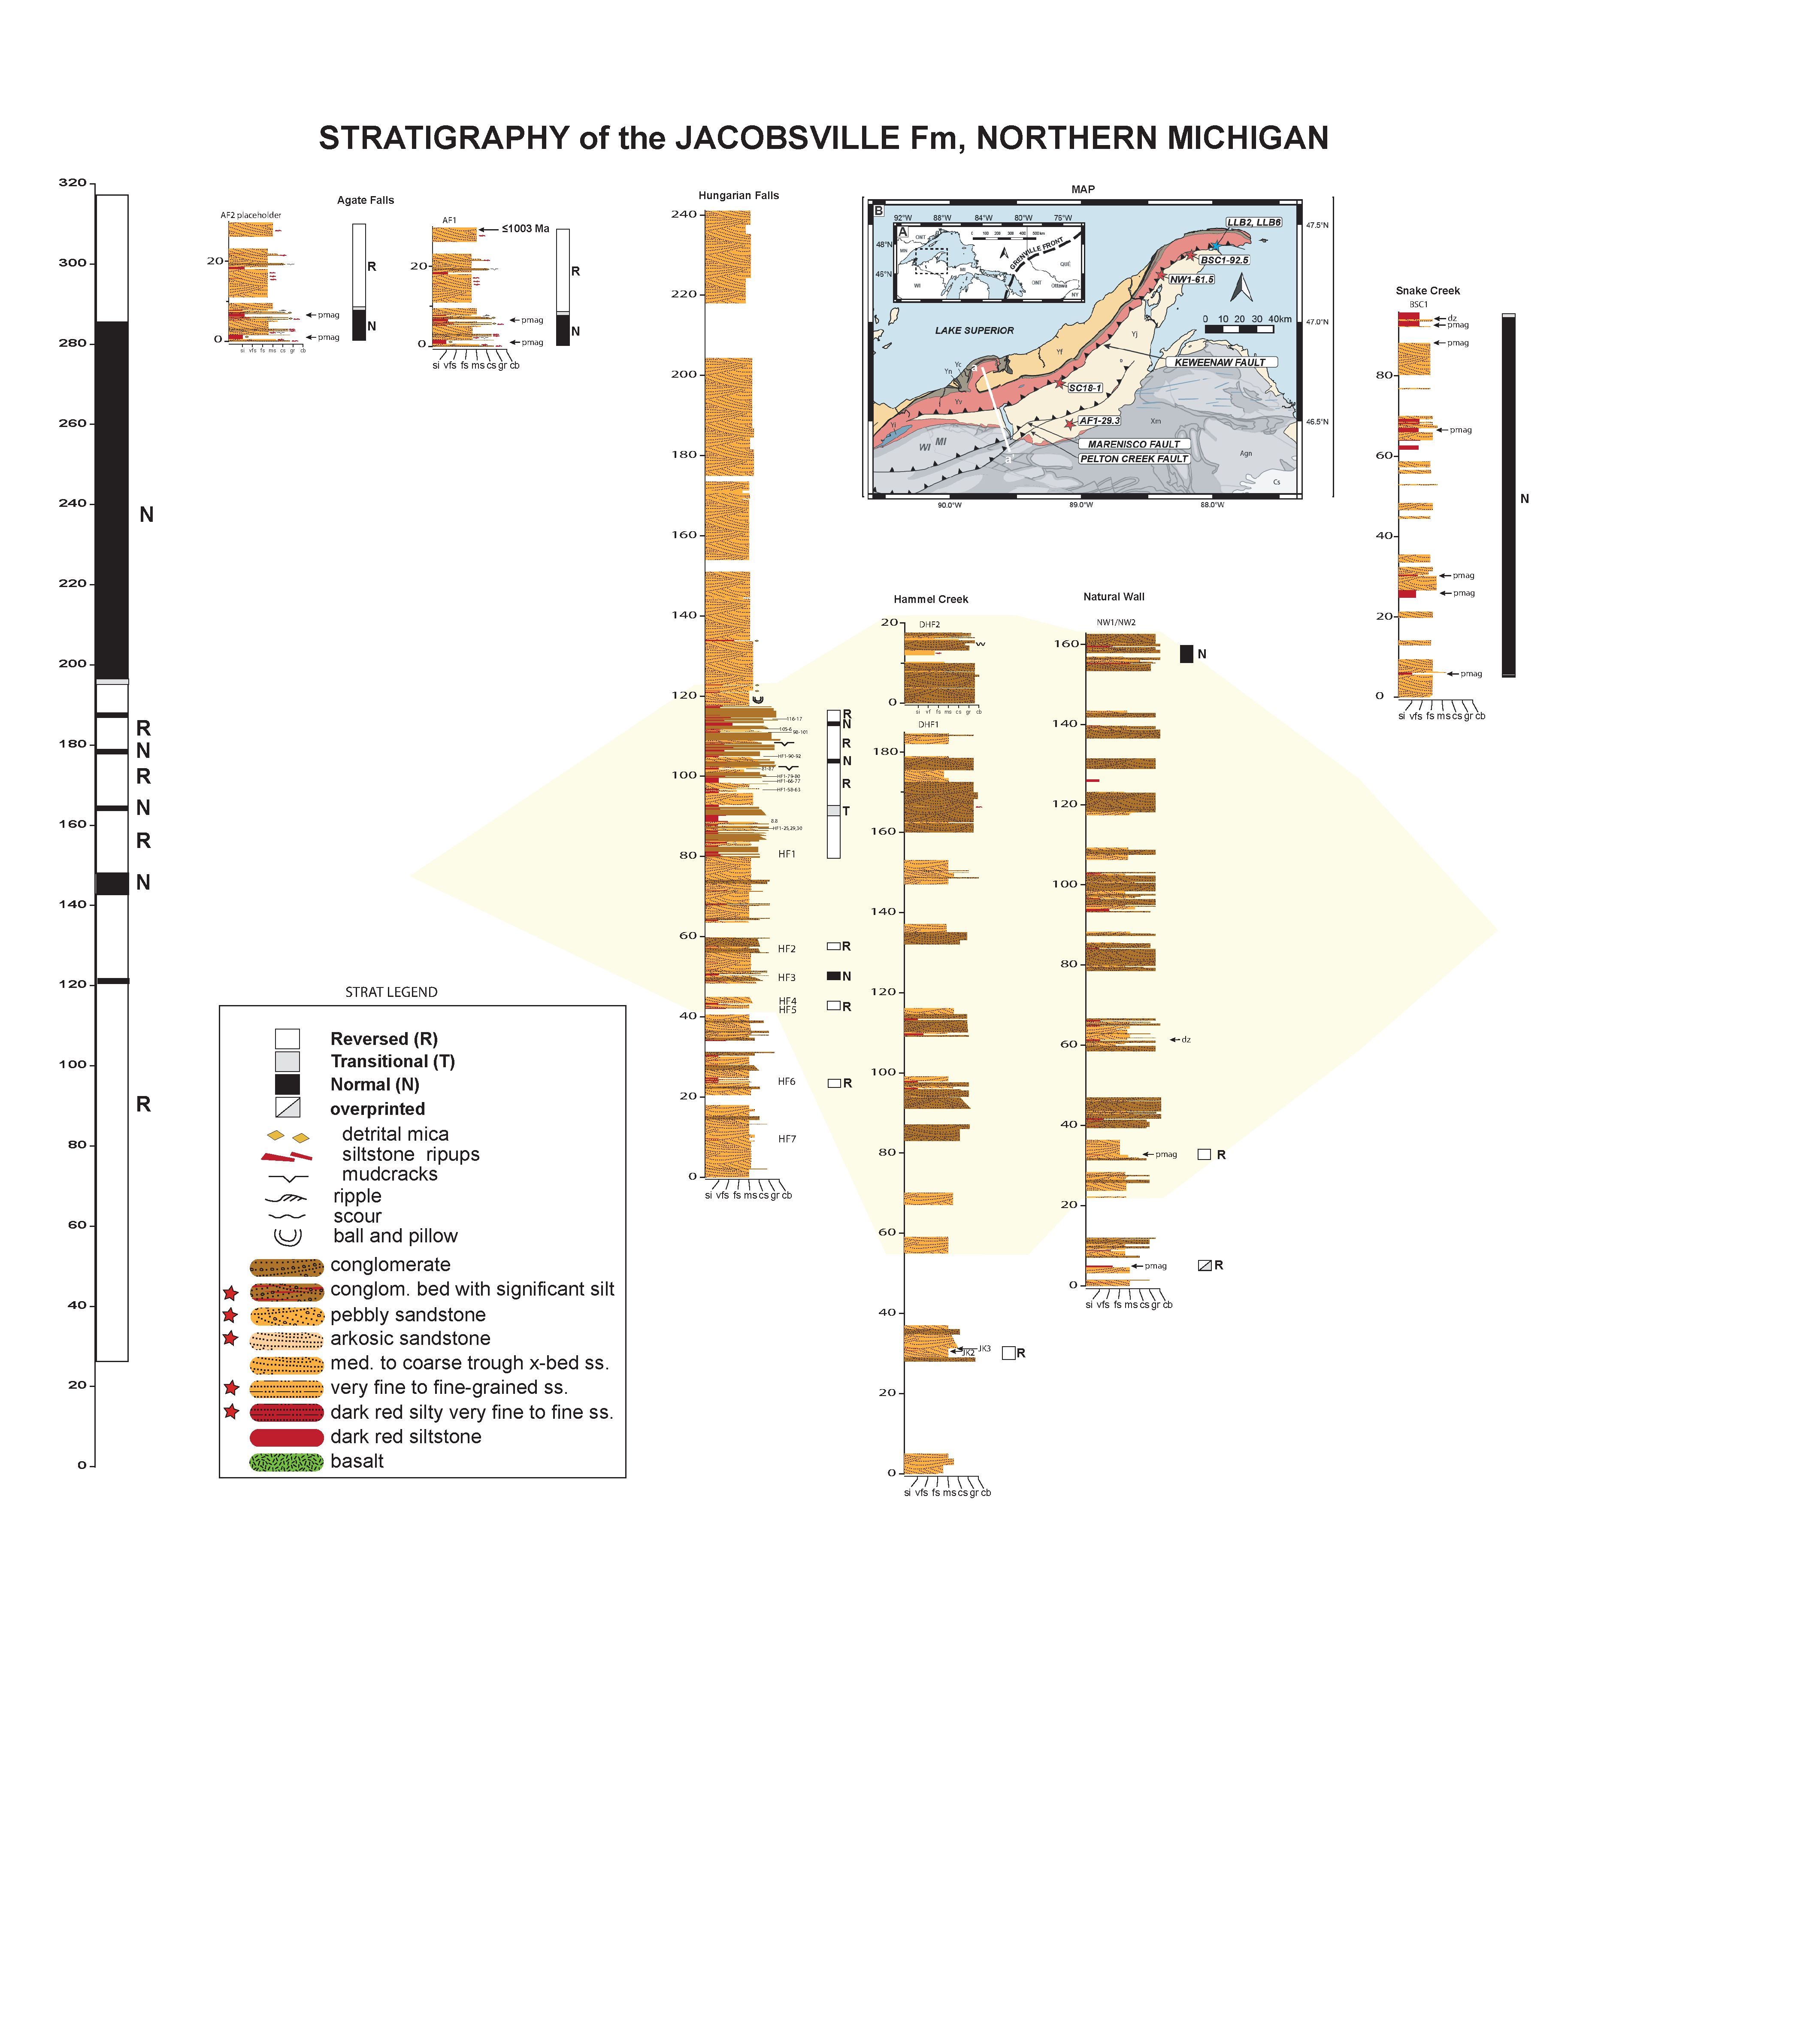
\includegraphics[width=0.9\textwidth]{Jacobsville_Sections_v3.pdf}
\caption{Tentative sedimentary stratigraphy and magnetostratigraphy for the Jacobsville Formation in northern Michigan, USA. Stratigraphic locations of paleomagnetic samples are shown in context of Jacobsville lithofacies, sedimentary structures, as well as detrital zircon maximum deposition ages developed by \citeA{Hodgin2022a}. }
\label{fig:strat_column}
\end{figure*}


% Blake's current tectonic model: after MCR volcanics ca. 1084 Ma emplacement follows the deposition of the sediments (Oronto Group) copper harbor conglomerate, Nonesuch formation and the Freda formation. Then the Grenville orogenesis took off with the Ottawan phase from 1020 Ma - 10?? Ma and the Rigolet phase from 995-980 Ma. Paleosol development and the unconformity between the Jacobsville and the volcanics indicate a prolonged period of gap during which the Oronto Group in the backbulge basin where they were deposited were lost, resulting in younger Jacobsville deposition directly on top of the volcanics. The fact that in the Jacobsville has conglomerate and sandstone and siltstone facies in them supports sediment input from the eroded Oronto Group. This indicate the older boundary of the Jacobsville deposition might be closer to the Rigolet Phase than the Ottawan phase. The younger age boundary of the Jacobsville is well defined - given that the maximum deposition age from the zircons of the Jacobsville is 993 Ma and the calcite on the Keweenaw Fault is 985.5 Ma, the deposition of at least the upper portion of the Jacobsville is well constrained to be between 993 and 985 Ma. The deposition of Jacobsville in the back bulge in Laurentia interior is related to the far-field compression caused by the Grenville Orogeny. 


\section*{Paleomagnetic results and inerpretation}

Oriented paleomagnetic samples were collected with a portable electric drill along five stratigraphic sections of the Jacobsville Formation in northern Michigan (Fig. \ref{fig:Geologic_map}, \ref{fig:strat_column}). Additional oriented cores and block samples of siltstone rip-up clasts within conglomerate lithofacies were sampled at Hungarian Falls and at Agate Falls (Fig. \ref{fig:Geologic_map}, \ref{fig:strat_column}). In order to maximize sampling of distinct time snapshots of the geomagnetic field at the time of Jacobsville deposition such that paleosecular variation can be sufficiently averaged, we optimized for vertical stratigraphic coverage such that each sample constitutes a paleomagnetic site considering that a paleomagnetic site (which ideally captures a single snapshot of the local geomagnetic field) is a particular bed in a sedimentary sequence. Red fine-grained sandstone to shaly siltstone layers were preferentially sampled as they tend to have lower permeability and are less susceptible to diagenetic alteration through fluid flow than coarser grained sandstone. Care was taken to avoid samples containing reduction spots. Paleomagnetic cores and blocks were oriented using a magnetic compass and a sun compass whenever possible. Sun compass data were preferentially used when available. A total of 379 specimens including 30 intraclasts where collected for paleomagnetic study. The specimens underwent stepwise thermal demagnetization at the UC Berkeley Paleomagnetism Lab using an ASC demagnetizer (residual fields $<$10 nT) with measurements made on a 2G DC-SQUID magnetometer. The demagnetization protocol had high-resolution approaching the Ne\'el temperature of hematite. As a result, 356 specimens yielded detrital remanent magnetizations that can be fitted with least-square lines. (5 \textdegree C to 2 \textdegree C) (Fig. \ref{fig:intraclast_pmag}). Demagnetization results are plotted in Figure \ref{fig:in_situ_pmag}A by locality. All paleomagnetic data are available to the measurement level in the MagIC database (https://earthref.org/ MagIC/; THIS LINK IS AVAILABLE TO REVIEWERS AND WILL BE UPDATED WHEN A DOI IS AVAILABLE).

\begin{figure*}[h!]
\centering
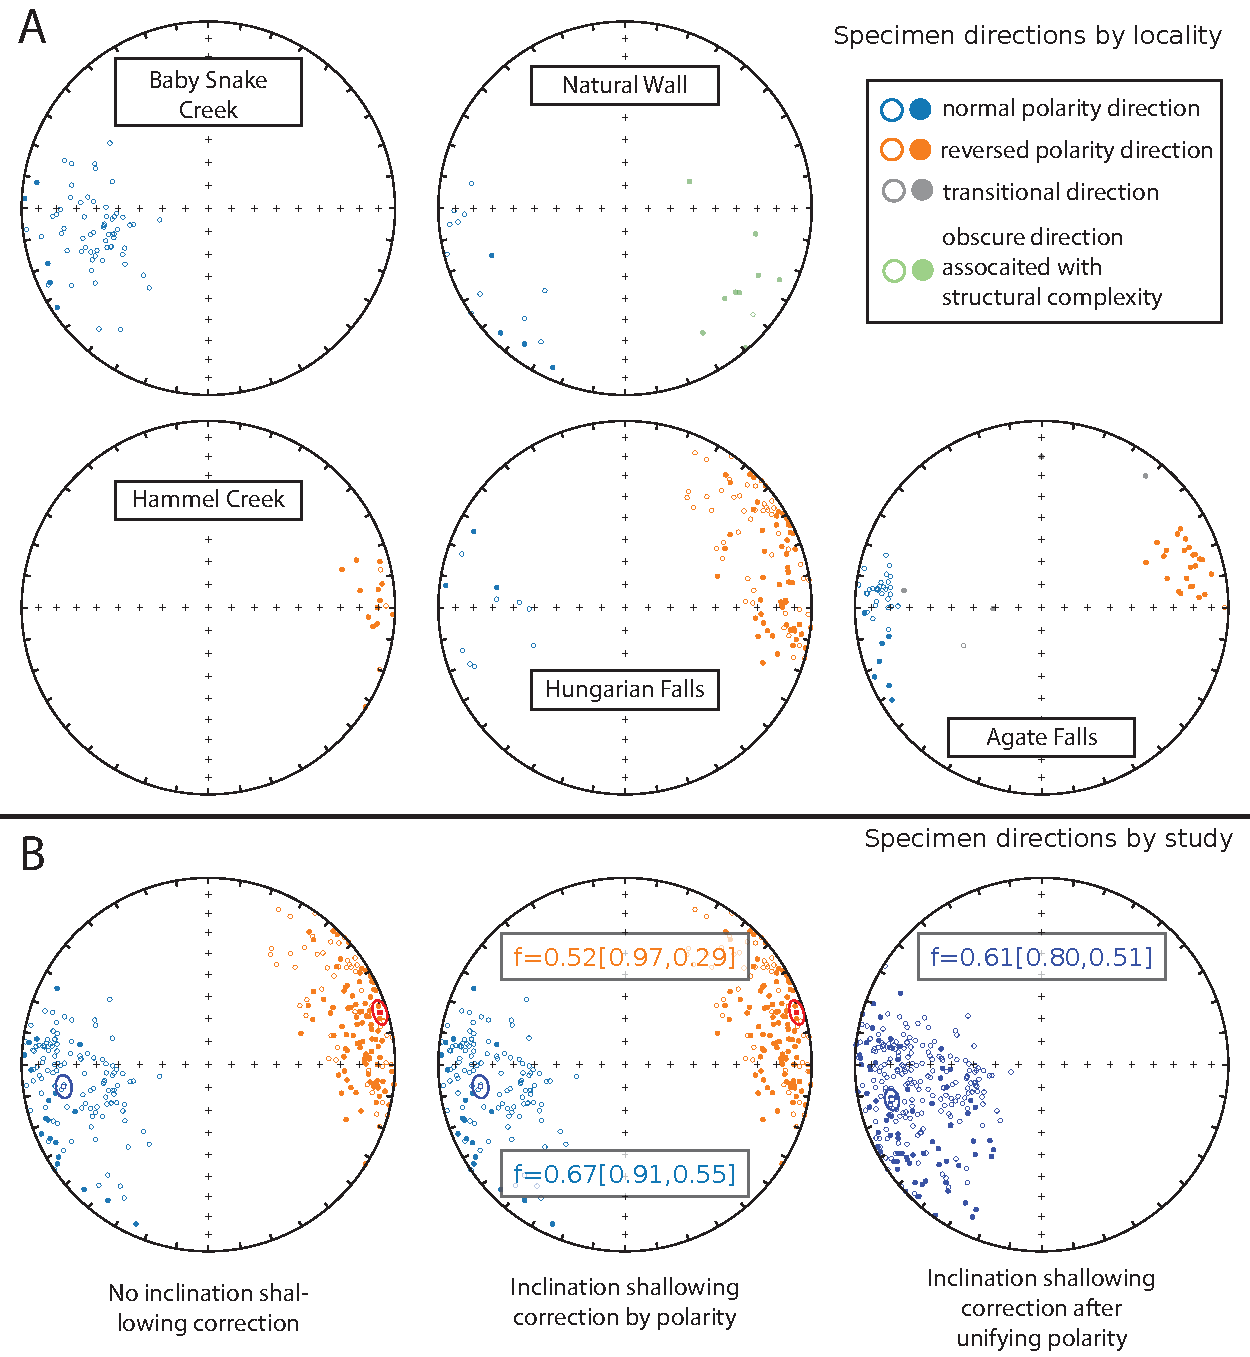
\includegraphics[width=\textwidth]{in_situ_pmag.pdf}
\caption{A) Specimen detrital remanence directions plotted by locality on equal area plots. During sample collection, we optimized for vertical stratigraphic coverage such that each sample constitutes a paleomagnetic site considering that a paleomagnetic site. B) Summary equal area plots at the study-level combining directions from all localities. The elongation/inclination (E/I) method \cite{Tauxe2004b} for estimating the amount of inclination shallowing in Jacobsville red beds are applied separately to specimen remanence directions of each polarity and to all specimen directions after flipping the reversed (orange) directions to their antipodes (blue). Details on inclination shallowing corrections are shown in Figure \ref{fig:EI_results}.}
\label{fig:in_situ_pmag}
\end{figure*}


\subsection*{Paleomagnetic field test}

\subsubsection*{Fluvial intraclast conglomerate test}

Similar to the thermal demagnetization result of the hematite-bearing fluvial intraclasts of the Freda Formation \cite{Swanson-Hysell2019b}, the siltstone rip-up clasts of the Jacobsville Formation typically reveal two distinct magnetization components (Fig. \ref{fig:intraclast_pmag}). One component show similar vector orientations amongst intraclasts and was typically removed up to 640-655 \textdegree C (Fig. \ref{fig:intraclast_pmag}). This indicates that it is likely a chemical remanent magnetization acquired through growth of secondary hematite in pore spaces following redeposition of the clasts. After removal of this component, further thermal demagnetization with small step increments at higher temperatures up to $\sim$689 \textdegree C often reveal an origin-trending component (Fig. \ref{fig:intraclast_pmag}). In the data from the clasts, there is typically a significant directional change in specimen magnetization between the mid-temperature component and the high-temperature component. As a result, 28 out of 30 intraclast specimens could be fit with distinct mid-temperature and high-temperature least squares lines \cite{Kirschvink1980a}. Distinct from the well-grouped mid-temperature component directions, the high-temperature directions of the intraclasts are dispersed and the null hypothesis of randomness cannot be rejected at the 95\% confidence level (n=6 for intraclasts at Agate Falls and n=22 for intraclasts at Hungarian Falls; Fig. \ref{fig:intraclast_pmag}; \citeA{Watson1956a}). This indicates that the remanence was acquired by detrital hematite grains during initial deposition of the grains.

\begin{figure*}[h!]
\centering
\includegraphics[width=\textwidth]{intraclast_pmag.pdf}
\caption{Paleomagnetic data from fluvial rip-up clasts of the Jacobsville Formation reveal a mid-temperature component that typically unblocks up to 655 \textdegree C and a high-temperature component that typically unblocks up to 689 \textdegree C. The components are present as varying fractions of the overall remanence as seen in the three individual clasts shown on vector orthogonal plots and measurement-level equal area plots in tilt-corrected coordinates (developed using PmagPy; \citeA{Tauxe2016a}). The direction of the mid-temperature component (interpreted as CRM) is shown as green arrows on the vector component plots and green circles on the equal area plots, while the high-temperature component (interpreted as DRM) is shown with purple symbols. The mid-temperature component has a similar direction among the clasts as can be seen on the summary equal area plots. In contrast, the high-temperature component directions (purple) are dispersed and pass a randomness test of \citeA{Watson1956a}. NRM = natural remanent magnetization; AFC = Agate Falls clasts; HFC = Hungarian Falls clasts.}
\label{fig:intraclast_pmag}
\end{figure*}

\subsubsection*{Fold test}

A total of 70 specimens yielded interpretable DRM directions throughout the stratigraphic section at Baby Snake Creek (Fig. \ref{fig:Geologic_map}, \ref{fig:in_situ_pmag}). 46 specimens were collected from the steeply tilted beds close to the Keweenaw fault and the rest 24 were from nearly horizontal beds. This allows us to conduct the paleomagnetic fold test on these specimens to investigate the timing of detrital remanence acquisition. A bootstrap fold test \cite{Tauxe1994a} result shows 95\% confidence bounds for the best grouping of the directions from the various beds of the fold is achieved between 55\% and 92\% unfolding (Fig. \ref{fig:fold_test}). Although the 95\% confidence bounds exclude both 100\% unfolding and geographic coordinates, the results indicate the directions are better grouped with a significant amount of tilt correction is applied complex folding regime such as non-cylindrical folding or multiple folding episodes about different axes could contributed to this fold test result not including 100\% unfolding within the 95\% confidence bounds.  

\begin{SCfigure*}
\centering
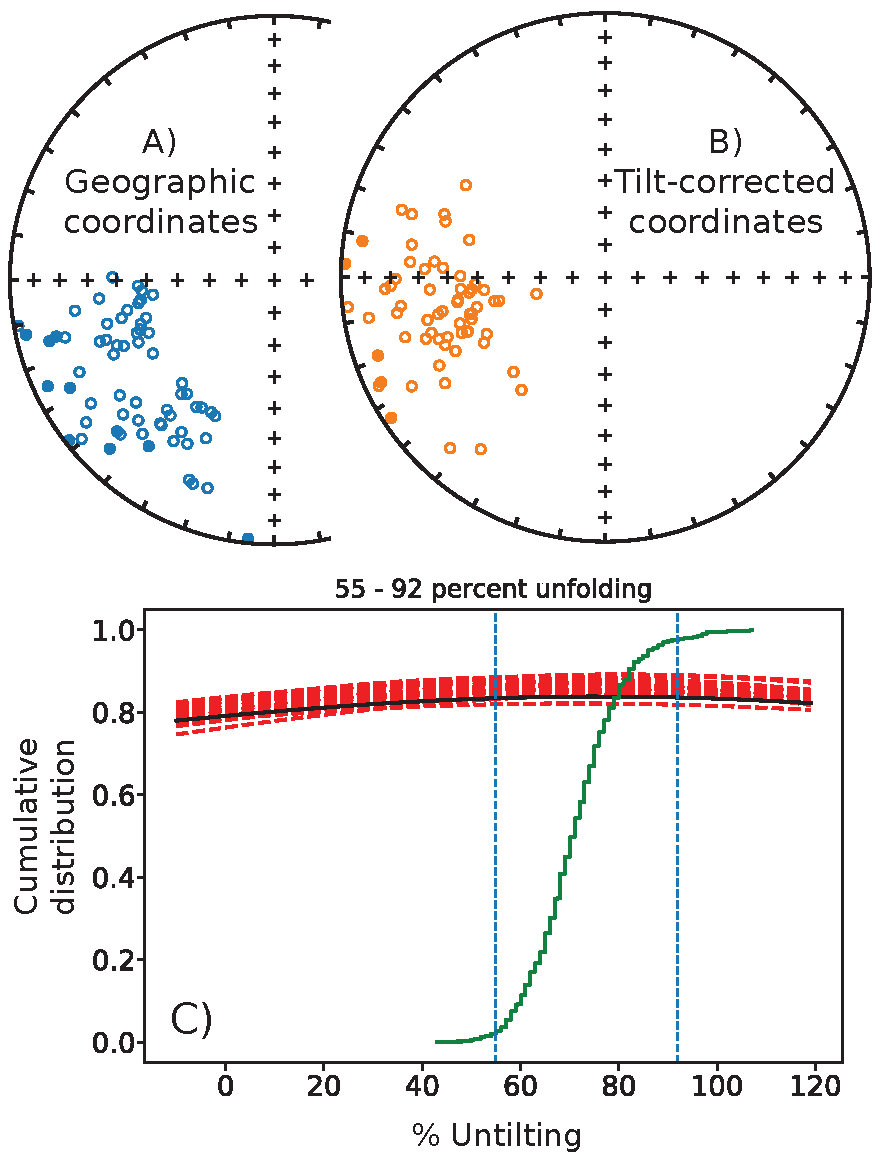
\includegraphics[width=0.5\textwidth]{SC1_fold_test.pdf}
\caption{Bootstrap paleomagnetic fold test \cite{Tauxe1994a} of the detrital remanent magnetization directions recorded by specimens from Baby Snake Creek. The directional data set becomes more tightly grouped than in geographic coordinates when applying 55\%-92\% unfolding, but both geographic and 100\% unfolded coordinate systems are excluded at the 95\% confidence level. }
\label{fig:fold_test}
\end{SCfigure*}

\subsection*{Tentative magnetostratigraphy}
\label{magstrat}
With the insights gained from the thermal demagnetization results of the Jacobsville fluvial intraclasts (Fig. \ref{fig:intraclast_pmag}), we next investigate the detrital remanent magnetizations for all in situ specimens that were collected along the five localities in northern Michigan (Fig. \ref{fig:Geologic_map}). The resultant DRM directions are plotted by locality in Fig. \ref{fig:in_situ_pmag}. These results show dual polarities with some specimens recording transitional field directions (Fig. \ref{fig:in_situ_pmag}), consistent with the observation of \citeA{Roy1978a}. While \citeA{Roy1978a} observed only one polarity reversal, our new data show that the Jacobsville Formation recorded multiple geomagnetic field polarity reversals. A tentative magnetostratigraphy is proposed in Fig. \ref{fig:strat_column}. In order to aid later discussions regarding the paleogeography of Laurentia, we refer to the westerly DRM directions as of normal polarity and the easterly DRM directions of reversed polarity (Fig. \ref{fig:in_situ_pmag}). 

At Hungarian Falls (Fig. \ref{fig:Geologic_map}), numerous hematite-rich siltstone to fine-grained sandstone layers were deposited (Fig. \ref{fig:strat_column}). Throughout $\sim$240 meters of strata, a total of 158 samples were collected for paleomagnetic study. At stratigraphic height of $\sim$24 meters (Fig. \ref{fig:strat_column}), 8 samples from a $\sim$0.5-meter-thick siltstone layer record reversed polarity directions (easterly declination and shallow inclination; horizon HF6). At stratigraphic level $\sim$42 meters (horizon HF5; Fig. \ref{fig:strat_column}), 4 samples were collected through a $\sim$0.2 m siltstone horizon including one specimen from near the base of the layer and three specimens near the top of the layer. The DRM component from the three specimens near the top all record a reversed polarity whereas the specimen collected near the base show a westerly direction. The westerly direction indicates that the geomagnetic field could have gone through a reversal between strata at 24 and 42 m, although more samples are needed to test the length and stability of the potential period of normal polarity. Therefore, we tentatively mark a period of transitional field near the base of horizon HF5 in Fig. \ref{fig:strat_column}. A reversed polarity field seems to have been maintained as 5 samples from horizon HF4 consistently record easterly directions just above the top of HF5 (Fig. \ref{fig:strat_column}). However, at least one geomagnetic field polarity reversal happened between the deposition of siltstone layers of HF4 and HF3, as 7 samples from HF3 all record normal-polarity directions. Subsequently, the field appears to flip again back to reversed polarity, as is shown by 7 samples from HF2 higher in the section (Fig. \ref{fig:strat_column}). Through the $\sim$35-meter-thick horizon of HF1 characterized by numerous siltstone to fine-grained sandstone layers interbedded with coarser-grained sandstone and conglomerate, magnetic polarity reversals of R-N-R-N-R were recorded (Fig. \ref{fig:strat_column}). 

The Natural Wall ravine and Hammell Creek are in close proximity to Hungarian Falls (Fig. \ref{fig:Geologic_map}) and the sedimentary facies characterized by trough cross-bedded sandstone and conglomerates are similar to the basal $\sim$120 meters of the section at Hungarian Falls (Fig. \ref{fig:strat_column}). Since only a few siltstone to fine-grained sandstone horizons were sampled at these two localities, we tentatively correlate the stratigraphic sections at these three localities based on their sedimentary facies (Fig. \ref{fig:strat_column}). At Hammell Creek, 14 samples from two siltstone layers near the base of the section are of reversed polarities, consistent with the reversed-polarity layers near the base of Hungarian Falls. Near the top of the Natural Wall section, consistent normal-polarity directions are recorded by 15 samples. This normal polarity is likely coeval with one of the normal-polarity periods recorded at Hungarian Falls, although it could indicate an additional polarity reversal from reversed to normal polarity that happened after the deposition of the youngest reversed strata at Hungarian Falls (Fig. \ref{fig:strat_column}). Near the base of the exposed stratigraphic section at Natural Wall (Fig. \ref{fig:strat_column}), the strata are steeply tilted or overturned (Fig. \ref{fig:Field_photo}). Tilt-corrected paleomagnetic directions from samples collected from these strata show dominantly southeasterly declinations that are distinct from either normal- or reversed-polarity directions higher along the strata or at Hungarian Falls. It is most likely that these directions resulted from noncylindrical or multiple episodes of complex folding. We hypothesize that these DRM directions were acquired during a reverse polarity episode similar to that recorded near the base of Hammell Creek (Fig. \ref{fig:strat_column}), but we will not include these directions in further paleomagnetic pole analyses. 

At Baby Snake Creek (Fig. \ref{fig:Geologic_map}), all 70 specimens that yielded interpretable high-temperature remanence have normal-polarity DRM directions \ref{fig:in_situ_pmag}). At Agate Falls (Fig. \ref{fig:Geologic_map}), multiple hematite-rich, detrital mica-bearing siltstone layers occur through a $\sim$30-meter strata incised by the running Middle Branch Ontonagon River. 68 paleomagnetic samples were collected on both sides of the waterfall (Fig. \ref{fig:strat_column}). A single transition from normal to reversed polarity is observed through the strata from bottom to top with a few strata in the middle of the section capturing transitional directions (Fig. \ref{fig:strat_column}, \ref{fig:in_situ_pmag}). 

Challenges exist in correlating the stratigraphic sections measured at the five localities in this study due to the lateral variability of the thickness of the formation associated with the variable paleotopographic relief of the Precambrian surface upon which the Jacobsville Formation was deposited \cite{Hamblin1958a, Kalliokoski1982a}. In particular, there may not be a unique solution in reconstructing the relative stratigraphic positions of the strata at Baby Snake Creek and Agate Falls with respect to the other three sections in central Keweenaw Peninsula due to geographical separation (Fig. \ref{fig:Geologic_map}, \ref{fig:strat_column}). However, at both Baby Snake Creek and Agate Falls, the sedimentary strata are dominated by siltstone to cross-bedded sandstone and are lacking significant amount of conglomerate facies as seen near Hungarian Falls. Given the relative facies abundance difference at these localities, an interpreted stratigraphic correlation could exist based on an interpreted sedimentary facies model. The conglomerates, hematite-bearing siltstones, and arkosic sandstones deposited near the Keweenaw fault could be associated with syn-depositional faulting that uplifted the Midcontinent Rift volcanics that subsequently eroded and shedded sediments near the fault. These facies, particularly the conglomerate facies, could have then been reworked and transported farther, resulting in the deposition of more sandstone-rich younger strata (Fig. \ref{fig:strat_column}). The relative lack of conglomerates at Agate Falls which is $\sim$25 km away from the Keweenaw fault could indicate that the Jacobsville sediments there are derived from far-travelled sediments. Recent field mapping near Baby Snake Creek have found evidence for the Jacobsville Formation onlapping the Midcontinent Rift volcanics that were previously faulted via en echelon segments\cite{Tyrrell2019a, Mueller2021a}. The unconformable contact between the sediments and the volcanics, instead of faulted contact typically observed near Hungarian could indicate that the deposition of the Jacobsville Formation near the northern end of Keweenaw Peninsula likely post-date some episodes of fault motion, and are thus younger than the sediments near the fault. Therefore, we interpret that the normal-polarity strata at Agate Falls and at Baby Snake Creek could be stratigraphically the youngest amongst the five localities, although a possibility that they instead are older strata deposited during the Keweenawan superchron \cite{Driscoll2016b} cannot be ruled out. 

Overall, the multiple geomagnetic field polarity reversals recorded by the Jacobsville Formation constrain the maximum range of the Keweenawan superchron \cite{Driscoll2016b} to be between ca. 1100 Ma (Mamainse Point Volcanics; \cite{Swanson-Hysell2019a}) to ca. 990 Ma (maximum deposition age of Jacobsville Formation; \cite{Hodgin2022a}). 

\section*{Discussion}

\subsection*{Inclination shallowing correction}

\begin{figure*}[H!]
\centering
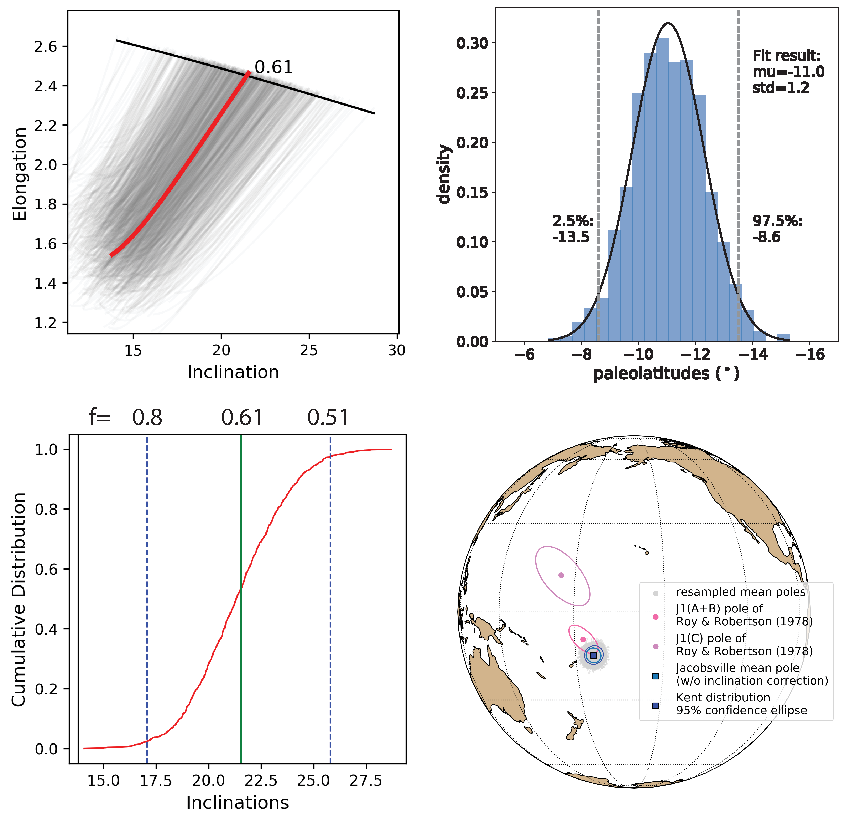
\includegraphics[width=\textwidth]{EI_results.pdf}
\caption{\footnotesize Results of the estimated amount of inclination shallowing of the detrital remanent magnetization of the Jacobsville Formation using the elongation/inclination (E/I) method \cite{Tauxe2004b}. Directions from both polarities are used with the reversed-polarity directions flipped to their antipodes (Fig. \ref{fig:in_situ_pmag}). A) The E/I method results in an estimated flattening factor $f$=0.61 (red curve) based on where elongation/inclination curve of the dataset intersects that predicted by the TK03 paleosecular variation model (black curve; \citeA{Tauxe2004b}). The grey lines show 1,000 bootstrap resamples of the DRM directions which provide an estimate of the uncertainty associated with the $f$ factor estimate. B) The distribution of the paleolatitudes implied from the resultant corrected inclinations from the E/I bootstrap resamples. That the distribution is drawn from a normal distribution with a mean of 11.0 and standard deviation of 1.2 cannot be rejected in the Kolmogorov-Smirnov test. The 95\% confidence bounds shown by dashed lnes span a range of paleolatitudes that need to be incorporated into the uncertainty of the reported paleomagnetic pole. C) The cumulative distribution of all plausible inclinations based on the E/I bootstrap results with the 95\% confidence bounds shown in inclination and $f$ value axes. D) Kent mean pole and Fisher mean pole of the Jacobsville Formation in context of previous poles from \citeA{Roy1978a} and the pole position derived from the Chequamegon Formation of the Bayfield Group developed by \citeA{McCabe1983a}. The mean pole position of the Kent distribution calculated from the distribution of resampled Jacobsville mean poles following the method of \citeA{Pierce2022a} overlaps with the Fisher mean pole position corrected by a single inclination shallowing value of 0.61. Both mean poles lie in between the Fisher mean poles calculated using the inclination-corrected normal and reversed pole groups respectfully. The close proximity between Jacobsville mean poles with the Chequamegon pole indicate their deposition could be largely coeval. The J1 (C) pole of \citeA{Roy1978a} is recorded by hematite-bearing sediments in Sault Ste Marie area. Its position in the northern hemisphere close to the Upper Freda Formation pole indicate that those sediment could be Freda-equivalent instead of Jacobsville-equivalent. $^*$---Fisher mean pole positions calculated with inclination shallowing correction given by the E/I results shown in Fig. \ref{fig:in_situ_pmag}. $^+$---the Freda Formation Fisher mean pole is corrected for inclination shallowing assuming $f$=0.6. }
\label{fig:EI_results}
\end{figure*}

Igneous and sedimentary rocks associated with the North American Midcontinent Rift provide high-resolution record of the ca. 1109 to 1070 Ma Keweenawan Track which tightly constrains the apparent polar wander path for Laurentia in the late Mesoproterozoic (Fig. \ref{fig:pole_plot}; \cite{Swanson-Hysell2019a}). However, high-quality paleogeographic constraints is lacking thereafter since magmatism in the interior of Laurentia entered a protracted quiescence period until the emplacement of the ca. 780 Ma Gunbarrel large igneous province \cite{Harlan2003a}. The new paleomagnetic pole developed from the Jacobsville Formation presents an opportunity to extend the APWP to the early Neoproterozoic as its maximum deposition age has been tightly constrained to be ca. 990 Ma through high-precision U-Pb detrital zircon geochronology and U-Pb calcite geochronology \cite{Hodgin2022a}. 

However, inclination bias associated with sedimentary paleomagnetic directions need to be corrected when synthesizing poles. Rotation of grains during sediment deposition and compaction during early diagenesis can result in the acquisition of a detrital remanent magnetization that is shallower than the local geomagnetic field in which it was acquired \cite{King1955a, Tauxe2005a, Kodama2012a}. This effect can be summarized as: 
\begin{equation*}
\textup{tan}(I_o) = f\textup{tan}(I_f)
\end{equation*}
where $f$ represents the amount of inclination shallowing, $I_o$ represents the observed inclination, and $I_f$ represents the inclination of the field in which the magnetization was acquired. If uncorrected, shallower inclinations obtained from sedimentary rocks can result in erroneously low estimates of paleolatitudes, biasing paleogeographic reconstructions \cite{Domeier2012a}. Methods for correcting sedimentary inclination bias include laboratory-based measurements of magnetic mineral fabrics \cite<e.g.>{Kodama1990a, Bilardello2015a}, as well as statistical methods based on the evaluation of the deviation of an observed virtual geomagnetic pole (VGP) distribution from that of a paleosecular variation model (the ``elongation/inclination" [E/I] method of \citeA{Tauxe2004b}). When a large number of sedimentary paleomagnetic sites (typically n$>$100) capture an extensive period of time such that the paleosecular variation is sufficiently averaged, the E/I method can give efficient estimates with reasonable uncertainty bounds via bootstrapping and is less labor-intensive than methods based on mineral fabric measurements. \citeA{Tauxe2009a} based on paleomagnetic data from lava flows of the North Shore Volcanic Group in the Midcontinent Rift to show that the ca. 1.1 Ga geomagnetic field had a behavior consistent with the prediction given by the TK03 paleosecular variation model of \citeA{Tauxe2004b}. \citeA{Pierce2022a} showed that the E/I method is effective in correcting the inclination bias recorded by a package of lava flow-bracketed fluvial red bed sediments---the Cut Face Creek Sandstone.

Inclination shallowing is also present in the fluvial red beds of the Jacobsville Formation. Scatter of the specimen detrital remanence directions in geographic coordinates show elongation of DRM directions parallel to the bedding plane, indicating the directions are shallowed (Fig. \ref{fig:in_situ_pmag}; \citeA{Tauxe2004b}). Since the deposition of the Jacobsville Formation span over geomagnetic field reversals, it is of interest to investigate the amount of inclination shallowing associated with the normal (n=130) and the reversed (n=148) polarity respectively (transitional fields and specimens affected by complex tilting regime are excluded). Applying the E/I method on the normal polarity directions yields an estimated $f$ value of 0.67 with 95\% bootstrap uncertainty bounds from 0.91 to 0.55 (Fig. \ref{fig:in_situ_pmag}B). Directions of reversed polarity yields an estimated $f$ factor of 0.52 with uncertainty bounds between 0.97 and 0.29 (Fig. \ref{fig:in_situ_pmag}B). Although the estimated $f$ value for the reversed-polarity directions has large statistical uncertainty bounds, the uncertainties are likely associated with the overall shallow inclinations and distributions of directions in both upper and lower hemispheres (Fig. \ref{fig:in_situ_pmag}B). Therefore, inclination corrections do not result in significant changes in the mean reversed direction. 

In addition, directions of the two polarities do not pass a reversal test \cite{McFadden1990a, Tauxe2010a}, regardless of whether inclination correction is applied. One interpretation of the asymmetric polarities could be that the deposition of the Jacobsville Formation was protracted such that the sediments at Hungarian Falls which dominate the reversed polarity records were deposited prior to those at Baby Snake Creek which dominate the normal polarity records (Fig. \ref{fig:in_situ_pmag}). This is consistent with our stratigraphic interpretation that Baby Snake Creek sediments could be younger than those near central Keweenaw Peninsula (i.e. Hungarian Falls, Natural Wall, Hammell Creek; Fig. \ref{fig:strat_column}). Other alternative interpretations could include that the mean poles are biased by transient non-dipolar fields due to insufficient averaging of paleosecular variation or transitional fields during field reversals. More data are needed to test these hypotheses. 

Overall, both inclination-corrected polarities recorded by the Jacobsville Formation show mean pole positions in the southern hemisphere with respect to today's continental configuration (normal polarity longitude=175.1\textdegree E, latitude=19.1\textdegree S, A95=3.8\textdegree; reversed polarity longitude=191.1\textdegree E, latitude=14.5\textdegree S, A95=3.9\textdegree; Fig. \ref{fig:EI_results}). The two pole positions are distinct from the youngest poles developed from rocks of the Midcontinent Rift (Fig. \ref{fig:EI_results}). Despite that the Jacobsville sedimentation span over geomagnetic field reversals, the large arc distance between either polarity of the Jacobsville Formation and the pole of the ca. 1070 Ma upper Freda Formation \cite{Henry1977a} is consistent with the interpretation that the onset of deposition of the Jacobsville Formation at the five studied localities post-date the youngest member of the Oronto Group sediments by tens of millions of years. 

% Field observations of \citeA{Tyrrell2019a} and \citeA{Mueller2021a} near Bete Grise Bay, which is only $\sim$10 km east to Baby Snake Creek (Fig. \ref{fig:Geologic_map}), show unconformable onlap of the Jacobsville Formation on top of Midcontinent Rift volcanics that have experienced significant thrusting, deformation. At some locations, paleosol development has been found on top of the Midcontinent Rift basalt along the segmented Keweenaw Fault branches prior to the deposition of the Jacobsville sediments. This is in contrast with the faulted contact between the Jacobsville Formation and the volcanics to the south where the Jacobsville Formation is often folded against the volcanics (Fig. \ref{fig:Geologic_map}). U-Pb calcite geochronology and thermometry confirm that the final $\sim$2 km vertical displacement along the Keweenaw Fault occurred during the ca. 980 Ma Rigolet phase of the Grenvillian Orogeny whereas the majority of the fault motion likely occurred during the ca. 1050 Ma Ottawan phase \cite{Hodgin2022a}. We interpret that it is most likely that deposition of the Jacobsville Formation initiated close to the Rigolet phase of the Grenvillian Orogeny with progressive sediment transportation to the northwest as the Grenville back-bulge basin propagated toward the interior of Laurentia \cite{Hodgin2022a}. As a result, we hypothesize that the sediments at Baby Snake Creek likely records a slightly younger pole position with a more southerly paleolatitude than those near Hungarian Falls, indicating Laurentia's plate motion toward the south (Fig. \ref{fig:EI_results}). However, we cannot rule out an alternative interpretation that the sediments at Baby Snake Creek are coeval or older than some of the sediments to the south, as the basal Jacobsville Formation at Baby Snake Creek is folded against the Midcontinent Rift volcanics. Further field mapping and geochronological constraints are needed to test this hypothesis. 



\subsection*{The Jacobsville paleomagnetic pole}

\begin{figure*}[h!]
\centering
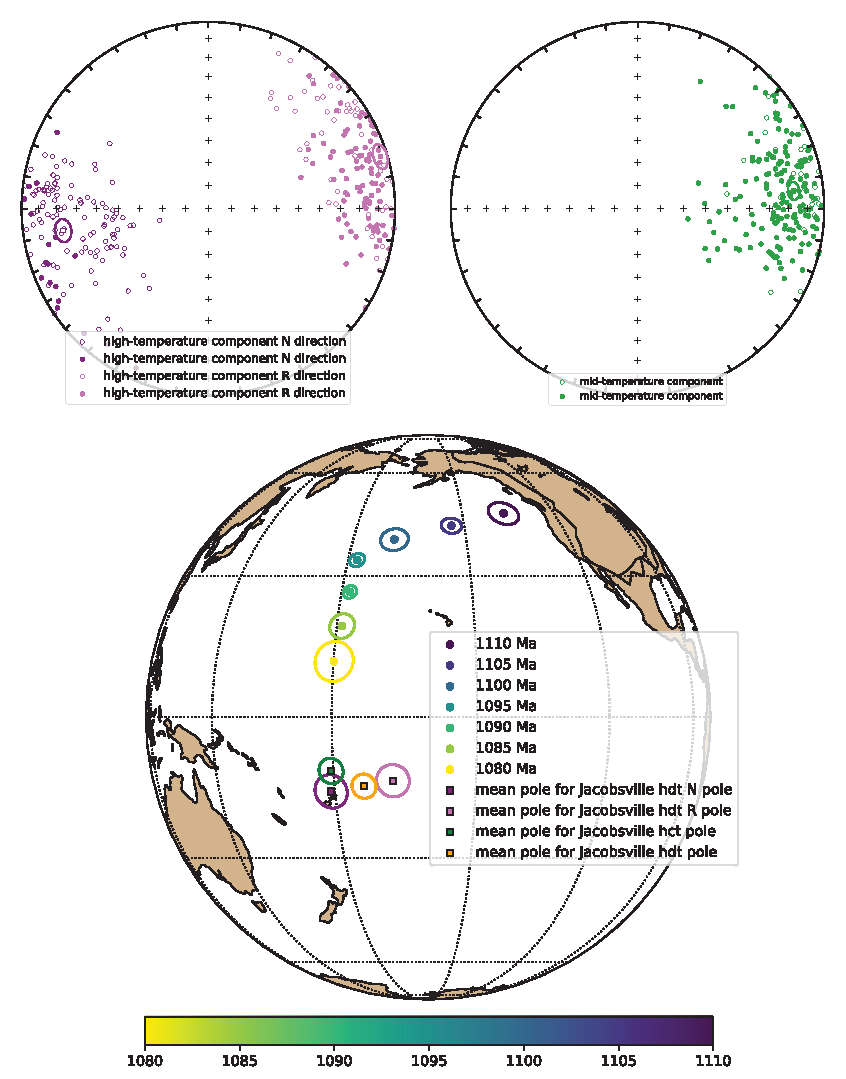
\includegraphics[width=\textwidth]{Jacobsville_pole_plot.pdf}
\caption{The Jacobsville Formation Kent mean pole position is plotted in context of the ca. 1109-1070 Ma Keweenawan Track (poles color-coded by age shown in the colorbar) and selected poles from the Grenville Province. The southerly pole position of the ca. 990 Ma Jacobsville Formation indicates Laurentia crossed the equator in the late Mesoproterozoic to early Neoproterozoic. The large arc distances between the Jacobsville pole and the poles of the Haliburton intrusions \cite{Buchan1976a} and the Wilberforce pyroxenite \cite{Palmer1973a} (black) indicate previous estimates of them being $>$1000 Ma \cite{Halls2015b} based on poor age and temperature calibration of their paleomagnetic and thermochronologic data are too old. \citeA{Brown2012a} developed poles (blue) from rocks of the Adirondack Mountains and estimated their ages to be ca. 960 Ma to 990 Ma, with the gneiss pole (lightest blue) being the youngest and the granites pole (darkest blue) being the oldest. However, the estimated closure temperatures for rutile was too low, biasing the estimated pole age to be too old. The true age of the Grenville poles could be much older than previously thought in light of paleomagnetic and chronological constraints from the Jacobsville Formation. }
\label{fig:pole_plot}
\end{figure*}

In light of the lithofacies model and detrital remanent magnetization data of the Jacobsville Formation, we prefer the interpretation that the deposition of the Jacobsville Formation initiated long after the the Oronto Group sedimentation and likely spanned a short time period close to the end of the ca. 1010 to 980 Ma Rigolet phase of the Grenville Orogeny \cite{Rivers2012a, Hodgin2022a}. Therefore, we combine DRM directions of both polarities of the ca. 990 Ma Jacobsville Formation to succinctly report one paleomagnetic pole for the formation. We reassess the amount of inclination shallowing of the combined directional dataset (Fig. \ref{fig:in_situ_pmag}). The resultant estimate for the $f$ value is 0.61 with a bootstrap 95\% uncertainty range for the $f$ value between 0.80 to 0.51, which overlaps with the uncertainty ranges of directions associated with either polarity (Fig. \ref{fig:in_situ_pmag}). The $f$ value of 0.61 is strikingly close to the value of 0.59 which is a calculated mean value of a compilation of inclination shallowing factor for hematite-bearing rocks derived by \cite{Bilardello2010b}. The Fisher mean paleomagnetic pole associated with the combined directions is shown in Fig. \ref{fig:EI_results} (pole longitude= 186.3\textdegree E, pole latitude= 14.3\textdegree S, A95= 2.5\textdegree). 

\citeA{Pierce2022a} discussed that as inclination shallowing processes usually do not bias the recorded declination, it would typically result in asymmetric uncertainties in the recorded paleomagnetic pole position with more uncertainties in paleolatitues than paleolongitudes. The asymmetric uncertainties in the mean pole position thus violate the assumption of the Fisher distribution \cite{Fisher1953a} where uncertainties are circularly distributed about a mean vector. Instead, the spherical asymmetric bivariate Kent distribution \cite{Kent1982a} is more appropriate for incorporating uncertainties associated with inclination shallowing in reported sedimentary paleomagnetic poles. We follow the approach of \citeA{Pierce2022a} who extended the E/I method of \citeA{Tauxe2004b}. First we take all estimated $f$ values from the bootstrap results of the E/I algorithm and apply each value to correct all Jacobsville detrital remanence directions (with the reversed directions flipped to antipodes). Then we calculate the Fisher statistics for each of the inclination-corrected mean pole. Finally, we perform a Monte Carlo approach to generate 100 resamples of each Fisher mean pole. As a result, the distribution of the resampled mean pole positions have an elongated distribution which represents more uncertainty associated with paleolatitudes of Laurentia than paleolongitudes (Fig. \ref{fig:EI_results}). The distribution of paleolatitudes of the resampled mean poles can be well-approximated by a normal distribution (Fig. \ref{fig:EI_results}). We use the Kent distribution to parameterize the 95\% confidence ellipse of the distribution of the resampled mean poles (mean longitude=186.4\textdegree E, mean latitude=14.2\textdegree S, major axis longitude=262.5, major axis latitude=43.5, major axis magnitude=3.3\textdegree, minor axis longitude=110.0, minor axis latitude=43.0, minor axis magnitude=3.0\textdegree; Fig. \ref{fig:EI_results}). As is shown in Fig. \ref{fig:EI_results}, although the Kent uncertainty ellipse has significant overlap with the circular uncertainty range calculated by the Fisher statistics due to the overall low paleolatitude of the Jacobsville basin, the Kent ellipse informs more uncertainty along the great circle path between the mean pole position and the locality of the basin as it incorporates the uncertainties in the amount of inclination shallowing within the sediments. 

\citeA{Roy1978a} isolated the detrital magnetization component via alternating-field, thermal, and chemical ``cleaning" demagnetization on a suite of Jacobsville red beds near Keweenaw Peninsula (their area A), the town of Marquette (area B), and Sault Ste Marie (area C). Although least-squares principal component analyses was not a routine approach in fitting paleomagnetic directions at the time, that study had success in removing the present day local field overprint and was able to resolve a magnetic polarity transition at one locality. The mean paleomagnetic pole position calculated from the interpreted primary magnetic remanence from rocks of the Keweenaw Peninsula and Marquette (J1 A+B pole; pole longitude=183\textdegree E, pole latitude=9\textdegree S, dp=3\textdegree, dm=6\textdegree; no inclination correction; Fig. \ref{fig:EI_results}; \citeA{Roy1978a}) is in the southern hemisphere and the uncertainty ellipse overlaps with that of the mean pole from this study (Fig. \ref{fig:EI_results}. However, their mean pole developed from red beds near Sault Ste Marie lies in the northern hemisphere with a latitude of 12\textdegree N (Fig. \ref{fig:EI_results}). Despite the large uncertainty ellipse associated with this mean pole position, it is distinct from the mean pole position from Jacobsville rocks in the Keweenaw Peninsula and Marquette. Instead, it overlaps with the mean poles of the ca. 1070 Ma Upper Freda Formation and the ca. 1075 Ma Nonesuch Formation (Fig. \ref{fig:EI_results}; \citeA{Henry1977a}). We hypothesize that the red beds collected by \citeA{Roy1978a} in Sault Ste Marie area are likely Freda-equivalent sediments, instead of being a part of the Jacobsville Formation. 

Deposition of the Bayfield Group sediments west to the Keweenaw Peninsula has been hypothesized to be coeval with the Jacobsville Formation but chronological constraints have been lacking \cite{Hamblin1958a, Kalliokoski1982a, Malone2016a}. Our new paleomagnetic data from the Jacobsville Formation confirm that the pole positions of the the Chequamegon Sandstone of the Bayfield Group and the Jacobsville Formation are close albeit distinct (Fig. \ref{fig:EI_results}). Given that the paleomagnetic pole from the Chequamegon Sandstone of the Bayfield Group (pole longitude=177.7\textdegree E, pole latitude=12.3\textdegree S, A95=4.6\textdegree; \citeA{McCabe1983a}) was calculated without applying inclination correction, the two formations could have an even closer temporal association than what appears in the current paleomagnetic pole configuration (Fig. \ref{fig:EI_results}). In addition, the fact that only reversed polarity directions were observed in the Chequamegon Sandstone indicate that deposition of the sandstone collected by \citeA{McCabe1983a} could be coeval with one of the reversed polarity periods recorded by the Jacobsville Formation (Fig. \ref{fig:strat_column}). To further test the temporal correlation between the sedimentary units, detailed paleomagnetic study and detrital zircon U-Pb geochronology data from the Chequamegon Sandstone are needed. 

\subsection*{Paleogeography of Laurentia in the late Proterozoic and the development of supercontinent Rodinia}

Constraining the paleogeography of Laurentia in the late Proterozoic is central to global paleogeography due to its central position in the ancient supercontinent Rodinia. During the initial assembly of Rodinia in the late Mesoproterozoic, Laurentia's apparent polar wander is well constrained by the ca. 1.1 Ga Keweenawan Track thanks to the large number of paleomagnetic poles paired with high-precision geochronology from rocks of the Midcontinent Rift \cite{Swanson-Hysell2019a}. Since the end of the Midcontinent Rift magmatism, well-dated paleomagnetic records from the the interior of Laurentia is lacking, and data from rocks associated with the ca. 1090 to 980 Ma Grenville Orogeny have been used to infer for Laurentia's plate configuration in the late Mesoproterozoic to early Neoproterozoic \cite<e.g.>{Weil1998a, Halls2015b}. However, in contrast to rocks of the Midcontinent Rift which usually have straightforward paleomagnetic records thanks to their simple thermal history \cite<e.g.>{Swanson-Hysell2019a}, rocks of the Grenville Province which experienced up to granulite facies metamorphism have much more complicated thermal histories and the timing of their magnetic remanence acquisition and alteration is more difficult to constrain. As is shown in Fig. \ref{fig:pole_plot}, paleomagnetic poles developed from rocks of the Grenvillian Orogeny plots near Australia with respect to today's continental configuration, forming arc distances ranging from $\sim$35\textdegree to more than 50\textdegree away from the pole of the ca. 1070 Ma Freda Formation \cite{Henry1977a}. Such large distance between pole positions associated with uncertainties in ages of Grenville magnetizations led to the controversial ``Grenville Problem"---did the Grenville rocks acquire magnetic remanence prior to the continental collision and thus the pole discrepancies are a result of significant crustal shortening (i.e. the ``two plate model"; \citeA<e.g.>{Irving1972a, Palmer1973a, Buchan1973a, Halls2015b}), or did they acquire remanence after the continental accretion and thus the southerly poles from the Grenville rocks represent a coherent plate motion through more recent times (i.e. the ``one plate model"; \citeA<e.g.>{Roy1978a, McWilliams1975a, Weil1998a})?

The two plate model is based on the interpretation that the Grenville rocks acquired magnetizations on allochthonous terranes in the late Mesoproterozoic, prior to the final accretion to Laurentia craton, resulting in their apparent southerly paleomagnetic pole positions today (Fig. \ref{fig:pole_plot}). Further, the lack of paleomagnetic poles in the southern hemisphere from interior Laurentia at this time (i.e. the Keweenawan Track) is further interpreted to support such allochthonous magnetic remanence hypothesis \cite<e.g.>{Warnock2000a, Halls2015b}. A corollary of such interpretation is that the Grenville paleomagnetic poles could record a large amount of crustal shortening associated with the Grenvillian Orogeny. \citeA{Halls2015b} suggested the lost crust must be up to 4000 $\pm$ 1000 km long.

Given the new constraints on the age and position of the Jacobsville pole (Fig. \ref{fig:pole_plot}), the two plate model would require that the majority of the crustal shortening happened during or after the Rigolet phase of the Grenville Orogeny, as the ca. 990 Ma Jacobsville pole is still $\sim$45\textdegree\ arc distance ($\sim$5000 km) away from the paleomagnetic pole of the Haliburton intrusions \cite{Buchan1976a} and $\sim$38\textdegree\ ($\sim$4000 km) from the pole of the Wilberforce intrusions \cite{Palmer1973a} (Fig, \ref{fig:pole_plot}). However, geologic and geochronologic evidence from both within the Grenville Province \cite{Aleinikoff2021a} and from interior Laurentia \cite{Hodgin2022a} indicate that majority of the deformation in the Grenville Province and the propagation of its compressional stresses into interior Laurentia happened during the ca. 1090-1020 Ma Ottawan phase orogeny, whereas smaller amount of convergence happened during the ca. 1010-980 Ma Rigolet phase. The lack of geological evidence for a striking amount of crustal shortening is consistent with the slow average plate motion between the deposition of the upper Freda Formation and the deposition of the Jacobsville Formation (average $\sim$0.2\textdegree/Myr; Fig. \ref{fig:pole_plot}). Therefore, it is kinetically unlikely that the plate of Laurentia suddenly increased its motion near the end of a collisional orogenesis in order to satisfy the Grenville pole positions. The plate kinetics interpretation based solely on paleomagnetic data and poorly constrained ages of magnetic remanence put forward by \citeA{Halls2015b} is implausible. 

Alternatively, the one plate model is much more straightforward in explaining the paleomagnetic pole positions of Grenville rocks as it interprets that those rocks acquired remanence during prolonged exhumation of the orogeny that postdate the peak metamorphism. In contrast to the two plate model, the one plate model would predict that ages associated with the Grenville poles are much younger than ca. 980 Ma (Fig. \ref{fig:pole_plot}). Adopting this model necessitates that the ages previously assigned to many Grenville poles be adjusted to much younger. Many previous paleomagnetic studies recognized that a large portion of the Grenville Province experienced up to granulite facies metamorphism (e.g. $>$700\textdegree C). The high metamorphism temperatures resulted in complete unblocking and overwriting of any previous remanence regardless of whether magnetite or hematite being the remanence carriers \cite<e.g.>{Ueno1975a, Alvarez1998a, Buchan1973a, Buchan1976a, Brown2012a}. However, what has not been fully taken into account in previous studies is the effective lowering of magnetic blocking temperatures of the new remanence. Theoretical calculations have shown that during prolonged cooling, magnetite which form above its Curie temperature (580\textdegree C) will subsequently acquire thermoviscous remanence \cite{Pullaiah1975a, Dodson1980a}, whereas hematite which often occur as exsolved lamellae in ilmenite in Grenville rocks acquired thermochemical remanence via magnetic ordering of the hemo-ilmenite below the Ne\'el temperature of hematite \cite{Burton1985a, Harrison2006b}. 

Due to the long time scales involved with thermoviscous and thermochemical origin of the magnetic remanence, it is not straightforward to interpret the natural blocking temperatures of Grenville rocks based on observations of unblocking temperatures in the lab where rocks are heated and cooled rapidly. \citeA{Brown2012a} studied Grenville rocks from the Adirondack Mountains. They recognized that the hemo-ilmenite exsolution occur at relatively low temperatures and acquire thermochemical remanence during cooling of the orogen and assigned an age of ca. 960 Ma to a paleomagnetic pole developed from hemo-ilmenite-bearing microcline gneiss from northwestern Adirondacks (Fig. \ref{fig:pole_plot}). Using the theoretical models of \citeA{Pullaiah1975a}, that study also extrapolated remanence ages of ca. 990 and ca. 970 Ma for the Wanakena granite and Marcy Massif anorthositic rocks whose dominant remanence carriers are magnetite grains that acquired thermoviscous remanence (Fig. \ref{fig:pole_plot}). However, in light of the ca. 990 Ma Jacobsville pole position and the slow down of Laurentia's apparent polar wander since ca. 1070 Ma, the ages assigned to the poles in \citeA{Brown2012a} could be still too old to be compatible with the magnetization being acquired after the major pulse of the orogenic collision. 

That the estimated ages associated with the Adirondack paleomagnetic poles are biased old can be attributed to the outdated thermochronometer closure temperature calculations of \citeA{Mezger1991a, Mezger1990a} whose data was used by \citeA{Brown2012a}. In particular, the cooling history for the Adirondack area estimated by \citeA{Mezger1991a, Mezger1990a} show that the orogen had cooled to $\sim$400\textdegree C by the time of U-Pb system closure in rutile crystals. However, this estimated U-Pb closure temperatures range for rutile was not based on laboratory Pb diffusion experiment, but instead was based on an assumption that thediffusion rate of Pb in rutile approximate that of Fe and Ti \cite{Mezger1989a}. Later experimental results \cite{Cherniak2000a} as well as analytical estimates \cite{Vry2006a, Kooijman2010a} show that diffusion rates of Pb in rutile are in fact much slower, indicating that previous calculations significantly underestimated closure temperatures of the system. Therefore, timing of magnetic remanence acquisition for Grenville rocks in the Adirondack Mountains should be younger than previously thought. 
The interpretation of young Grenville poles is supported by high-precision U-Pb apatite thermochronology data from iron oxide-apatite deposits of the eastern Adirondack Mountains \cite{Krestianinov2021a} and from the Wilberforce pyroxenite of the Wilberforce region, Canada \cite{Paul2021a}. Apatite from both regions yield ages of ca. 900 Ma with associated closure temperatures $\sim$450\textdegree C \cite{Cherniak1991a, Chamberlain2001a}. Considering delayed remanence acquisition of magnetite and hematite, ca. 900 Ma should be closer to the actual timing when rocks of the Grenville Province finally blocked in their remanence that is preserved today. However, the exact age of each paleomagnetic pole recorded by rocks of different domains of the Grenville Province remains largely uncertain. Complications such as the origin of the dated iron oxide-apatite ore, crystal-size dependence of closure temperature of accessory minerals including rutile and apatite \cite{Smye2018a, Chamberlain2001a}, and the complex metamorphic histories in different domains of the Grenville Province require that more high-precision thermochronology data with modern closure temperature calibration are developed. 

Overall, albeit that numerous paleomagnetic data has been developed from rocks of the Grenville Province, few are paired with high-precision thermochronology data that are calibrated by modern diffusion paramters. More high-precision thermochronology data and statistical models that properly incorporates uncertainties associated with timing of closure of thermochronometers and with magnetic remanence acquisition temperatures in the slowly cooled orogen are needed in order to further calibrate the age of those poles. Further development of paired pole-age data from the rich suite of metamorphic rocks in the Grenville Province can help update Laurentia's APWP \cite{Irving1974a} and the paleogeographic configuration of super continent Rodinia in the Neoproterozoic.  


\section*{Conclusion}

Our new paleomagnetic pole from the ca. 990 Ma Jacobsville Formation passes paleomagnetic field tests and has robust radiometric age constraints. This high-quality pole is a crucial addition to Laurentia's apparent polar wander path in the late Proterozoic. It extends the Mesoproterozoic Keweenawan Track (Fig. \ref{fig:pole_plot}) by showing that the plate slowed down significantly as the Grenville collisional orogenesis commenced on Laurentia's margin. It also sets an anchor for the position of supercontinent Rodinia in early Neoproterozoic due to Laurentia's central position in the configuration. Being a robust record from rocks in interior Laurentia, the Jacobsville pole implies that ages associated with the paleomagnetic poles recorded by metamorphic rocks of the Grenville Province might need to be adjusted significantly. Further paired studies of high-quality paleomagnetism and high-precision thermochronolgy are needed to illuminate Laurentia's development toward mid Neoproterozoic and its connection with conjugate continents such as Baltica. 


\section*{Data Availability}
Paleomagnetic data associated with this study are available within the MagIC database (\url{XXX}; UPDATE WHEN DOI IS GENERATED) and all data are within a Github repository associated with this work (\url{https://github.com/Swanson-Hysell-Group/Jacobsville}) that is also archived on Zenodo (\url{https://doi.org/XXX}). This repository also contains Python code that implements all of the calculations, visualizations and statistical tests discussed herein. 

\acknowledgments
This project is funded by NSF grant EAR-1847277 to Nicholas Swanson-Hysell. 

\bibliography{YZ_ref}


\end{document}
